\documentclass[twocolumn]{article}
\usepackage{amsmath}
\usepackage{float}
\usepackage{pgfplots}

\providecommand{\keywords}[1]{\noindent \textbf{\textit{Keywords}} #1}
\bibliographystyle{unsrt}

\pgfplotsset{
    legend entry/.initial=,
    every axis plot post/.code={%
        \pgfkeysgetvalue{/pgfplots/legend entry}\tempValue
        \ifx\tempValue\empty
            \pgfkeysalso{/pgfplots/forget plot}%
        \else
            \expandafter\addlegendentry\expandafter{\tempValue}%
        \fi
    },
}

\begin{document}

\title{Eventually Consistent Partying}
\author{Veit Heller}

\maketitle

\begin{abstract}
In distributed systems and life in general, eventual consistency is the
desirable state of agreement. In this paper, we show how to reach this state in
the context of parties with regards to the buzz factor (also known as
inebriation quotient).
\end{abstract}

\bigskip

\keywords{Party System Design, Buzz Factor, SIGBOVIK}

\section{Introduction}

In classical distributed systems, eventual consistency is a state of agreement
between nodes in a system that is reached at a certain point in time. This
property is usually desirable because it provides clear grounds on which to
base assumptions about the state of the system.

At parties, too, there is a certain state of agreement—or agreeability, if you
will—that is usually beneficial to the mood of the actors in the system, a
property worth optimizing for. This property is in strong correlation with the
buzz factor—also known as inebriation quotient—, which describes the state of
alcohol saturation of a given actor.

In this paper, we describe a novel approach to reason about eventual
consistency as it relates to partying.

\section{Preliminaries}

Our foremost goal for eventual consistency in a party setting is reaching a
quorum of approximate buzz level. It is said to be almost impossible to set up
a perfectly consistent system unless you set up a group of exclusively sober
actors. There is no consensus on whether a group of sober actors can be
classified as a party in the literature, as some authors prefer to call those
systems “tea parties”.

We characterize an actor by their buzz intake behaviour and their buzz
threshold. If the buzz threshold is reached, we characterize an actor as having
dropped out and disregard them when checking for a quorum. The buzz threshold
seems to be correlated to the actor’s gender, age, and bodyweight.

At this stage, it is important to note that there is no standard unit that
allows us to talk about buzz-related activities. For the purposes of this paper,
we will assume the standard unit to be “one can of beer (Fat Tire Amber Ale)”.
Interested parties suggested the authors use the more well-known unit of “one
can of beer (Bud Light)”, but that idea was quickly discarded because the
authors had doubt that a credible party could be based on said unit.

The sole medium of buzz accounted for in this paper is ethanol. While other
substances seem to be in use for party-related buzzing, describing their
respective interrelations would complect the calculations tremendously while
accounting only for a reasonably small subset of actors.

\subsection{Archetypes}

In our research we discovered four primary archetypes of actors at parties in
relation to attaining the buzz factor. We will describe them in the following.

\paragraph{Serious Business.} Actors in the “Serious Business” class—also known
as “winos” or “boozehounds”—are characterized by a quick intake of buzz.
Depending on their buzz threshold, they might drop out early.

\paragraph{Dead Sober.} Actors in the “Dead Sober” class—also known as
“buzzkills” or “designated drivers”—do not intake buzz. Accordingly, they either
have to be in the majority to achieve what is known as an \textit{a priori}
quorum, or be in the minority, in which case they will work against the quorum
of the other actors.

\paragraph{Low and Slow.} The “Low and Slow” class of actors—also known as
“normies”—shows a slow, steady intake of buzz. Any spikes in buzz may be
counteracted by the intake of water or other non-alcoholic substances, though
the increase of buzz over time is almost inevitable.

\paragraph{Sugar Rush.} Favoring Cocktails and longdrinks, this class of
actors—also known as “fancypants” or “amateur baristas”—show almost no signs of
buzz for a period of time—this period is unpredictable and largely based on the
compounds used when intaking buzz—before a sudden spike of buzz that can easily
overshoot the buzz threshold. That point in time is known as “the tipping point”
in the literature, and will be referred to as such in the following.

\bigskip

While this collection of archetypes is helpful in building a vocabulary for
expressing actor behavior, it should not be taken as canonical or exhaustive.
Party architecture is an understudied area of systems design, and we expect many
novel, more accurate categorizations to emerge in the coming years.

\section{Practical Discussion}

Now that we have laid the groundwork to conceptualize the system, we will
develop a vocabulary of basic buzz-related calculations.

\subsection{Calculating the Buzz Factor}

We have found that a reasonable way to calculate the buzz factor is to presume
that there exists a function \texttt{f} that, given a time \texttt{t}, returns
the buzz intake at that time. Calculating the total buzz factor at any given
point in time is then as simple as taking the sum of buzz intakes from
\texttt{t0}—being the time at which the party started—to \texttt{t1}—being the
time for which the buzz factor should be calculated.

When accounting for each actor independently, it is important to adjust \texttt{f} based on their archetype. The model of the archetype might need to
be adjusted slightly to account for the individual differences between actors
within the same archetype category. Machine Learning algorithms might be able
to predict better versions of \texttt{f} for an actor given behavior samples
during previous parties, though that area has heretofore been vastly
understudied.

In the following we shall give an overview of functions that seem to best
predict actor behavior per archetype. Note that the buzz threshold cannot be
predicted and needs to be measured or assumed by the architect.

\paragraph{Serious Business.} Actors in this class should best be modelled by a
function that returns a static value, since their buzz factor is usually
monotonically increasing. An increase by one unit of measurement per hour can
usually be assumed. When accounting for individual actors, that number might
change, also in accordance with the buzz factor, since some actors in this class
seem to drink more or less depending on their current inebriation quotient.

\begin{figure}[H]
\[ f(t) = 1 \]
\caption{\texttt{f(t)} for “Serious Business”.}
\end{figure}

\paragraph{Dead Sober.} The function that describes this class of actors will
always return \texttt{0}.

\begin{figure}[H]
\[ f(t) = 0 \]
\caption{\texttt{f(t)} for “Dead Sober”.}
\end{figure}

\paragraph{Low and Slow.} This class of actors are modelled similarly to actors
of the “Serious Business” archetype, with the caveat that, as the party goes on,
they might occasionally lower their buzz factor. A base likelihood of
\texttt{1/3} can be chosen, meaning that once every three units the buzz
factor will be reduced rather than increased. This process can be made to
seem more “lifelike” by introducing random or even fandom numbers
\cite{fandom}. It is also reasonable to assume a slower buzz intake of about
half a unit per hour.

\begin{figure}[H]
\[ f(t) =
  \begin{cases}
    -0.2       & \quad \text{if } t \text{ is evenly divisible by 3}\\
    0.5        & \quad \text{otherwise}
  \end{cases}
\]
\caption{\texttt{f(t)} for “Low and Slow”.}
\end{figure}


\paragraph{Sugar Rush.} A lot of work on party systems design has been devoted
to modelling the actors in this class, and for good reason. While the actor
count of this archetype across the entire population seems to be smaller than
that of the “Low and Slow” archetype, for instance, all functions modelling
their buzz intake have been the subject of a high level of scrutiny in the
party architecture community, since none of them have yet seemed to fit a
majority of actors. A combination of two positive values, one for the time
values before the tipping point, and one for the time values after the tipping
point, has led to promising results. The tipping point varies, but an average of
four hours into the party seems to be a reasonable assumption.

\begin{figure}[H]
\[ f(t) =
  \begin{cases}
    0.2       & \quad \text{if} t < 4\\
    1.5       & \quad \text{if} t \geq 4
  \end{cases}
\]
\caption{\texttt{f(t)} for “Sugar Rush”.}
\end{figure}

\subsection{Modelling a Party}

To model a party, the current buzz factor of each actor that has not dropped
out—i.e. each actor whose buzz factor is below their buzz threshold—must be
calculated. A quorum of buzz factors is reached when a majority of actors have
approximately the same buzz factor, where approximate means a distance of not
more than 1.5 units of measurement between each actor.

\subsubsection{Example}

Let us model an eight hour long party of four people as an example. The
attendees consist of one designated driver of the “Dead Sober” archetype, two
normies in the “Low and Slow” category, and one wino who means “Serious
Business”. There is no actor of the “Sugar Rush” archetype present because the
host forgot to buy Ginger Ale and limes.

Choosing a reasonable buzz threshold for each actor, using the standard
functions from above, and graphing the results, we end up with a figure that
clearly shows that we have a quorum at the hours 1-4, after which point the
buzz factors diverge by more than 1.5 units between the designated driver and
the normies.

\begin{figure}[H]
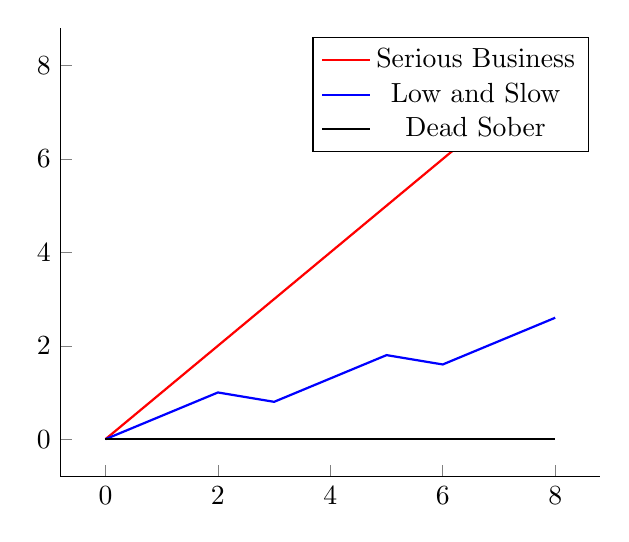
\begin{tikzpicture}
 \begin{axis}[axis lines*=left,domain=0:8]
  \addplot[no marks,thick,color=red, legend entry=Serious Business] {x};
  \addplot[no marks,thick, color=blue, legend entry=Low and Slow] plot coordinates {
    (0, 0)
    (1, 0.5)
    (2, 1)
    (3, 0.8)
    (4, 1.3)
    (5, 1.8)
    (6, 1.6)
    (7, 2.1)
    (8, 2.6)
  };
  \addplot[no marks,thick, legend entry=Dead Sober] {0};
 \end{axis}
\end{tikzpicture}
\caption{A party, graphed.}
\end{figure}

\section{Conclusion}

Party systems design is a nascent, but promising field. We believe that by
introducing ideas from the wider world of distributed systems the field can
develop a better vocabulary and more rigorous design methods which will
eventually lead to a higher quality of parties.

\bibliography{eventually_consistent_partying}

\end{document}
